\documentclass[ headinclude,footinclude]{scrbook}
\usepackage{xeCJK}
\usepackage[adobefonts]{ctex}
\usepackage[a4paper]{geometry}
\usepackage{ragged2e}
\usepackage{titletoc}
\usepackage{amsmath}
\usepackage[dvips]{xcolor}
\usepackage{tikz}
\usepackage{listings}
\usepackage{graphicx}        % standard LaTeX graphics tool
\usepackage{float}
\usepackage{tocloft}
%\usepackage{fancyhdr}
\usepackage[
%nochapters, % Turn off chapters since this is an article        
eulermath,% Use the Euler font for mathematics
%pdfspacing, % Makes use of pdftex’ letter spacing capabilities via the microtype package
dottedtoc % Dotted lines leading to the page numbers in the table of contents
]{classicthesis}
\usepackage{arsclassica}
\usepackage[strict]{changepage}
\usepackage{titlesec}
\usepackage{fontspec}
\usepackage[T1]{fontenc} 
\usepackage{xcoffins}
\strictpagecheck

\def\mytitle{中德文化差异小百科}
\def\mytext{Projekt4}

\definecolor{halfgray}{gray}{0.55}%定义所需颜色
\definecolor{titlepagecolor}{cmyk}{1,.60,0,.40}

\definecolor{RoyalBlue}{cmyk}{1,.60,0,.40}

\newfontfamily\mybold{FZXingKai-S04}
\newfontfamily\myregular{Alegreya-Regular}
%\newfontfamily\dinprolight{AlegreyaSans-Light}

\DeclareFixedFont{\titlefont}{T1}{ppl}{b}{bt}{0.4in}
% Set up commands for title page generation
\definecolor{ethblue}{RGB}{31, 64, 122}


\graphicspath{ {image/} }

\makeatletter                       
\def\printauthor{%                  
	{\large\@author}}              
\makeatother

\author{%
	\center
	\textbf{Chinesisch-Deutschen Institut für Angewandte Ingenieurwissenschaften (CDAI)} \\	
	\vspace*{1em}
	\texttt{http://cdai.zust.edu.cn/}
}

% The following code is borrowed from: https://tex.stackexchange.com/a/86310/10898

\newcommand\anglei{-45}%定义角度
\newcommand\angleii{45}
\newcommand\angleiii{225}
\newcommand\angleiv{135}
%绘制版面镶边代码
\newcommand\chapterdecoration{%
	\begin{tikzpicture}[remember picture,overlay,shorten >= -10pt]
	\coordinate (aux1) at ([yshift=-15pt]current page.north east);
	\coordinate (aux2) at ([yshift=-410pt]current page.north east);
	\coordinate (aux3) at ([xshift=-4.5cm]current page.north east);
	\coordinate (aux4) at ([yshift=-150pt]current page.north east);
	\checkoddpage
	\ifoddpage
	\else
	\coordinate (aux1) at ([yshift=-15pt]current page.north west);
	\coordinate (aux2) at ([yshift=-410pt]current page.north west);
	\coordinate (aux3) at ([xshift=4.5cm]current page.north west);
	\coordinate (aux4) at ([yshift=-150pt]current page.north west);
	\renewcommand\anglei{-135}
	\renewcommand\angleii{135}
	\renewcommand\angleiii{-45}
	\renewcommand\angleiv{45}
	\fi
	\begin{scope}[halfgray!40,line width=12pt,rounded corners=12pt]
	\draw
	(aux1) -- coordinate (a)
	++(\angleiii:5) --
	++(\anglei:5.1) coordinate (b);
	\draw[shorten <= -10pt]
	(aux3) --
	(a) --
	(aux1);
	\draw[opacity=0.6,halfgray,shorten <= -10pt]
	(b) --
	++(\angleiii:2.2) --
	++(\anglei:2.2);
	\end{scope}
	\draw[halfgray,line width=8pt,rounded corners=8pt,shorten <= -10pt]
	(aux4) --
	++(\angleiii:0.8) --
	++(\anglei:0.8);
	\begin{scope}[halfgray!70,line width=6pt,rounded corners=8pt]
	\draw[shorten <= -10pt]
	(aux2) --
	++(\angleiii:3) coordinate[pos=0.45] (c) --
	++(\anglei:3.1);
	\draw
	(aux2) --
	(c) --
	++(\angleiv:2.5) --
	++(\angleii:2.5) --
	++(\anglei:2.5) coordinate[pos=0.3] (d);
	\draw
	(d) -- +(\angleii:1);
	
	\filldraw[line width=0,rounded corners=0] (0,3) rectangle (\linewidth,3.05);
	\end{scope}
	\end{tikzpicture}%
}

\titleformat{\chapter}[display]%
{\normalfont\Huge\sffamily}%
{{\color{halfgray}\chapterNumber\thechapter%
		\hspace{10pt}\vline} }{10pt}%
{\spacedallcaps}[\vspace*{3cm}\chapterdecoration]

\begin{document}
	\pagestyle{empty}
	\NewCoffin \result
\NewCoffin \anchor
\NewCoffin \topbox
\NewCoffin \ethlogo
\NewCoffin \imagebox
\NewCoffin \textbox
\NewCoffin \departmentlogo
\NewCoffin \textboxtext
\NewCoffin \textboxsubtext
\NewCoffin \authortext

\SetHorizontalCoffin \result {}
\SetHorizontalCoffin \topbox {\color{ethblue}\rule{220mm}{3cm}}
\SetHorizontalCoffin \imagebox {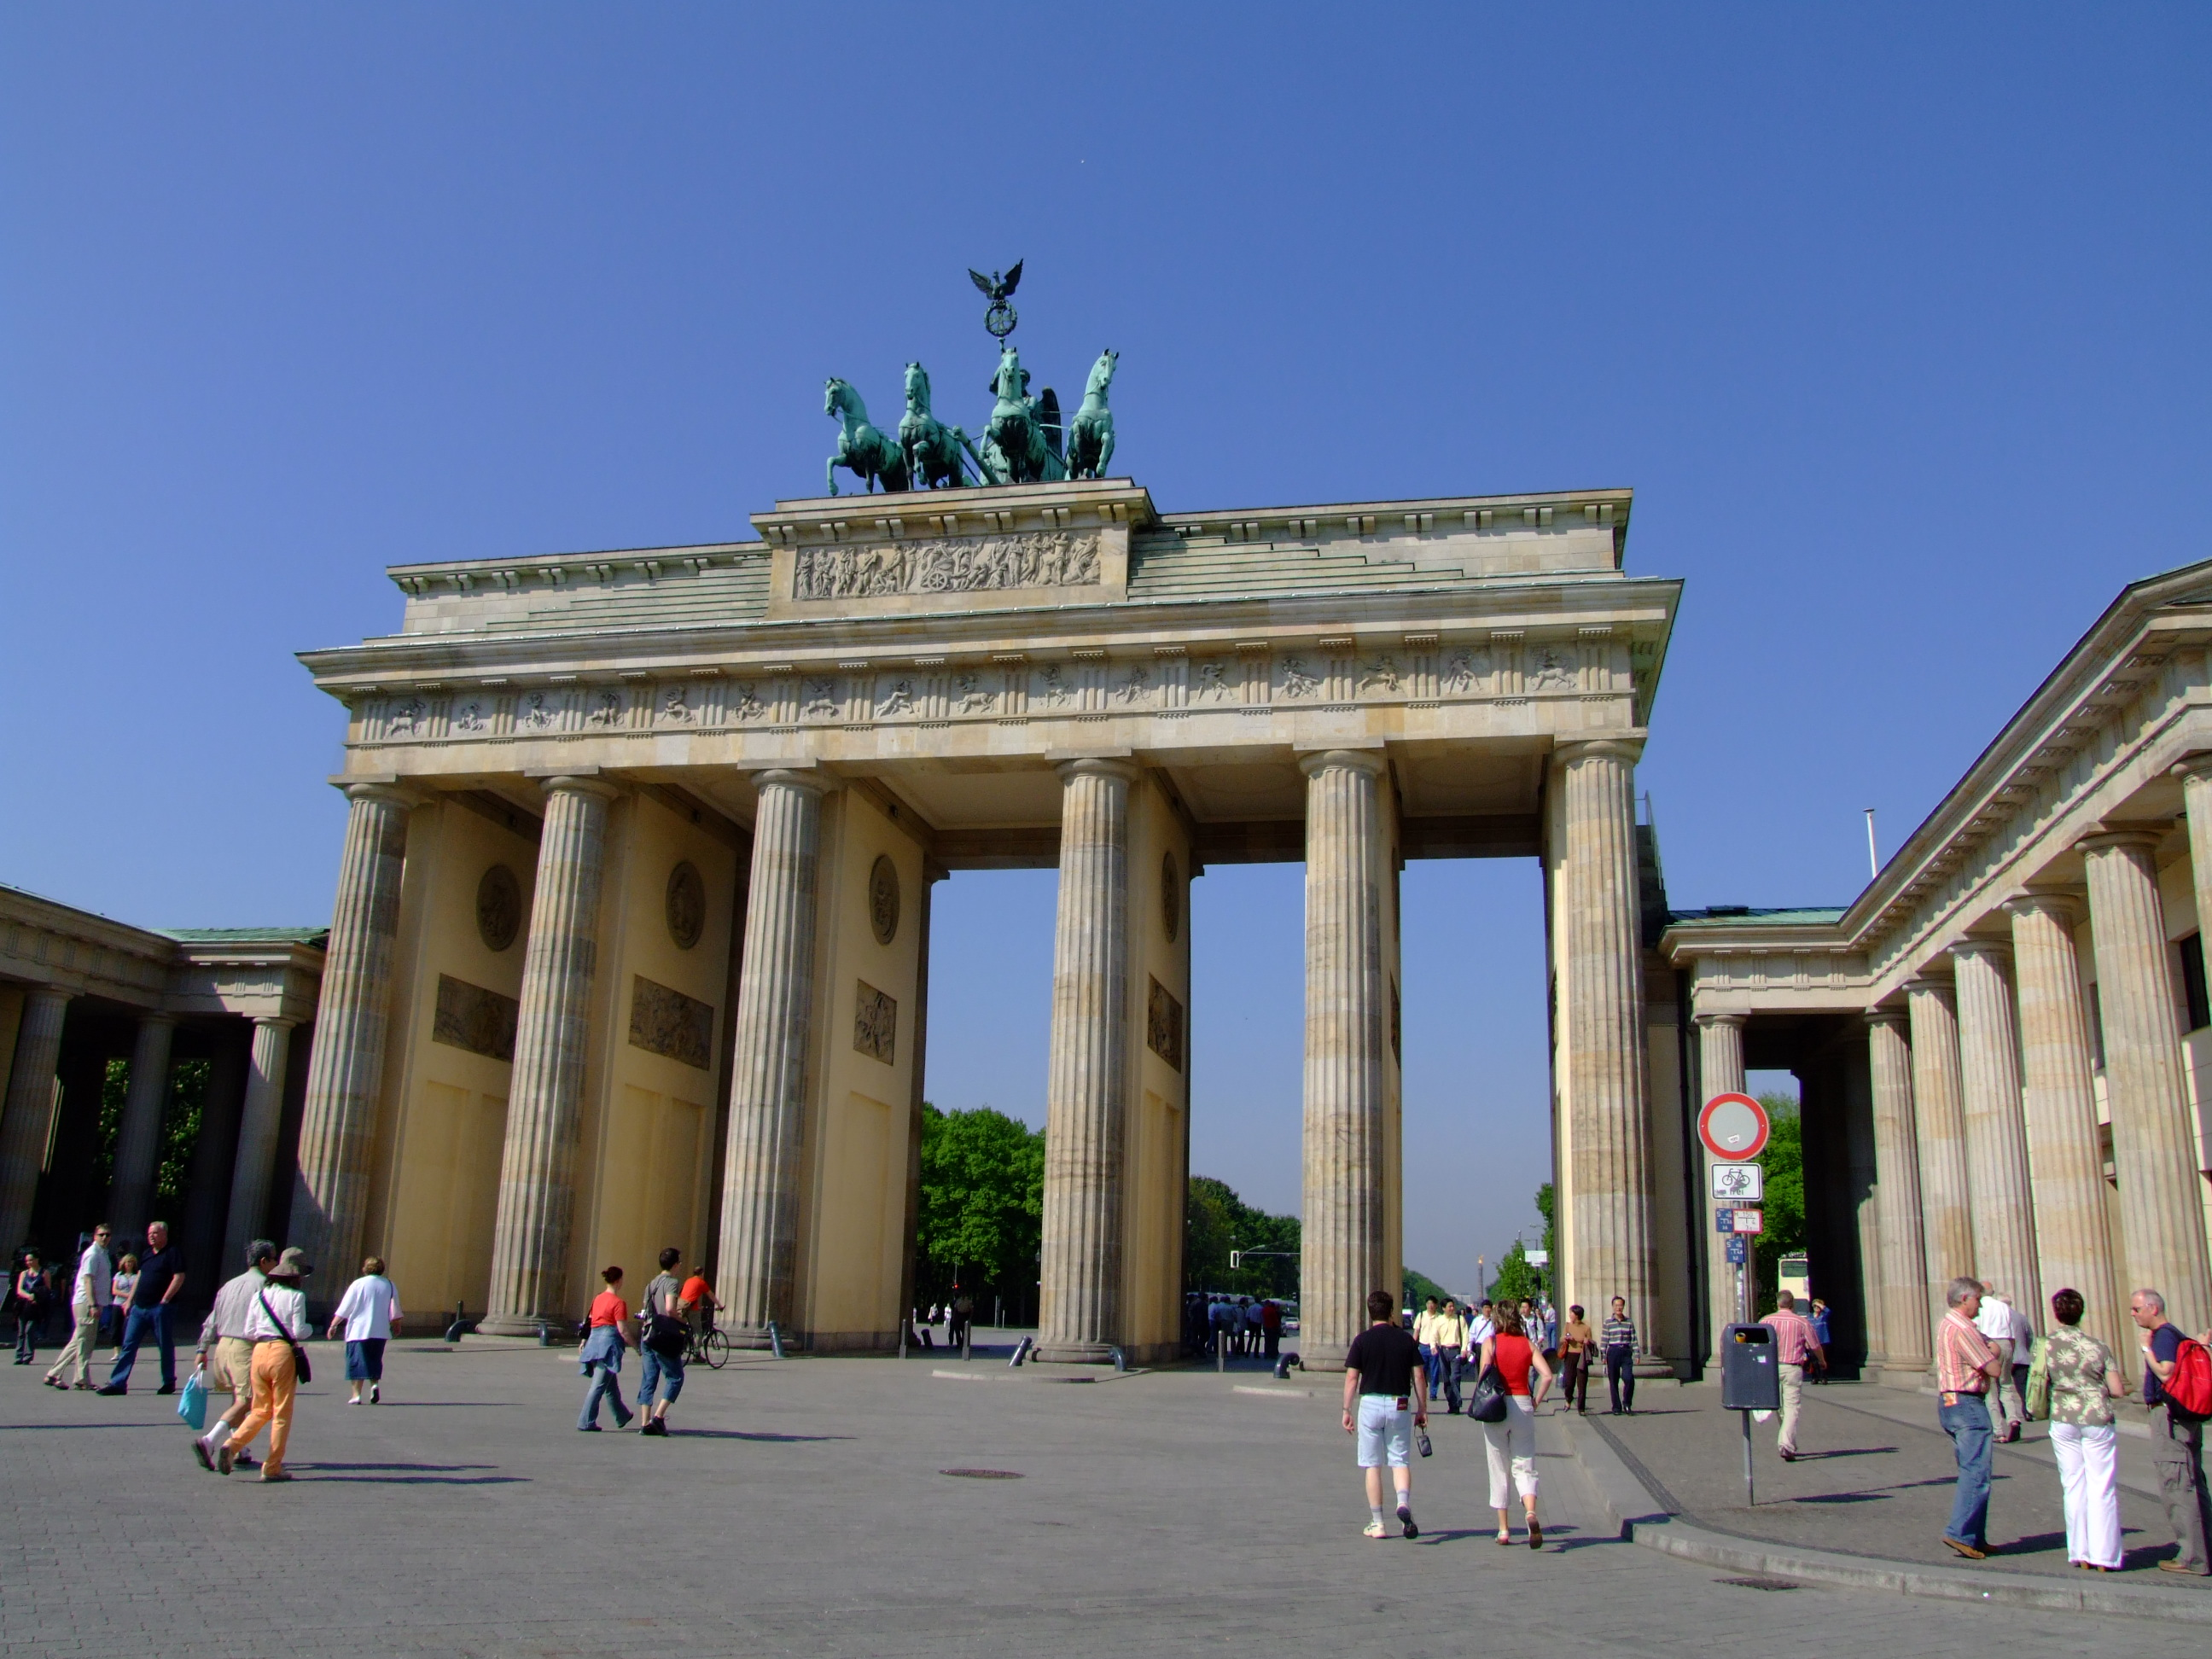
\includegraphics[width=190mm]{haupt}}
%\SetHorizontalCoffin \ethlogo {
\includegraphics[width=50mm]{logo}}
\SetHorizontalCoffin \textbox {\color{ethblue}\rule{190mm}{100mm}}
\SetVerticalCoffin \textboxtext {160mm} {\fontsize{40}{48}\mybold\noindent\textcolor{white}{\mytitle}}
%\SetVerticalCoffin \textboxsubtext {160mm} {\fontsize{21}{25}\dinproregular\noindent\textcolor{white}{MSc Thesis \\ Month Year}}
\SetVerticalCoffin \authortext {160mm} {\flushright\fontsize{21}{25}\myregular\noindent\textcolor{white}{\mytext}}
\SetHorizontalCoffin \departmentlogo {
\includegraphics[width=30mm]{logo}}

% Positioning Hax
\JoinCoffins \result \topbox
\JoinCoffins \result[\topbox-hc, \topbox-b] \imagebox [hc, t](0mm,10mm)
\JoinCoffins \result[\imagebox-l, \imagebox-t] \ethlogo [l, b](0mm,5mm)
\JoinCoffins \result[\imagebox-l, \imagebox-b] \textbox [l, t](0mm,0mm)
\JoinCoffins \result[\textbox-hc, \textbox-t] \textboxtext [hc, t](-5mm, -5mm)
\JoinCoffins \result[\textboxtext-l, \textboxtext-b] \textboxsubtext [l, t](0mm, -5mm)
\JoinCoffins \result[\textbox-r, \textbox-b] \authortext [r, b](-5mm, 5mm)
\JoinCoffins \result[\textbox-l, \textbox-b] \departmentlogo [l, t](-5mm, -5mm)


% Generate the page
\thispagestyle{empty}
\newgeometry{left=0mm,bottom=0mm, top=0mm, right=0mm}
\noindent\TypesetCoffin \result
\restoregeometry
	\newpage
	\begin{titlepage}
		\vspace*{6cm}
		\noindent
		\center
		\titlefont \mytitle \par
		\null
		\vspace*{12.5cm}
		\noindent
		\hfill
		
		\begin{minipage}{\linewidth}
			\center{\printauthor}
		\end{minipage}
	\end{titlepage}
	\newpage
	\renewcommand{\cftdot}{$\cdot$}
	\renewcommand\thefigure{\thesection-\arabic{figure}}
	\renewcommand\thetable{\thesection-\arabic{table}}
	\newcommand{\mypar}{\par\noindent}
	\setlength\parskip{0.7em}
	\makeatletter
	\@addtoreset{table}{section}
	\makeatother
	\makeatletter
	\@addtoreset{figure}{section}
	\makeatother
	
	\begin{minipage}{\linewidth}
\Huge\sffamily\center {Zu diesem Buch} \par
\end{minipage}
\thispagestyle{empty}
 \vspace*{3cm}
 %\normalfont\normalsize
 %\raggedright
 %\indent
 中国和德国都是世界上具有重大影响力的国家,随着传播 通讯技术的改进,交通技术的进步和经济的高度全球化,两国的合作越来越频繁。 然而,由于文化背景的不同,两国人民在交往的过程中不能够相互理解,,导致交际不能顺利进行。针对中德工程师学院和德国的应用技术大学之间日益频繁的交流活动,作为中德工程师学院的学生我们希望将一些所闻所知的一些信息整理、归类,尽可能为两国的学生做一些提示。本书不求包罗万象,但求准确,详尽,有趣。
\par
中德工程师学院(CDAI)于五月初在吕贝克大学和西海岸与科技(州)的浙江大学代表组成的会议上启动。经过浙江省政府的成功评估和中国教育部的认可,CDAI将在2014/2015冬季学期主办第一批中国学生。 CDAI是石勒苏益格 - 荷尔斯泰因州与浙江省长期成功合作的基础。该研究所的重点是石勒苏益格 - 荷尔斯泰因院校应用型本科工程项目: - 应用科学海德西海岸大学的管理和技术,以及 - 土木工程在FH吕贝克。约杭州三分之一的技术课程由各自的母校支持。教学语言最初是中文,从第三学期开始增加德语,从第三学期开始用德语授课。学习课程的成功参与者将获得德语和中文学士学位。对于最优秀的学生,可以切换到相应的德国应用科学大学三个学期,以完成他们在那里的学习。作为回报,来自合作大学相应学位课程的德国学生将完成他们在杭州的部分学业。
\par
 在上学期,我们小组成员在项目发起人Frau Schneider的引领和指导下,为了增进我院及合作院校中、德两国学生间的文化认同感,减轻乃至消除文化差异所带来的沟通障碍,同时也为了我院新生能够更快适应和融入国际化的教学方式,多元化的人文环境,开展了一系列关于中德文化差异的研讨会、采访、问卷调查和现场调研。我们最终决定将项目的视角聚焦在七个文化主题上:服饰、饮食、体育、工作、交通、文化、卫生,以Wiki为载体,以百科全书式的写作手法,从学生的视角出发,独特地展现出我们对于异国文化的认识与思考。在项目期间,我们充分运用所学项目管理的知识,通过Projekt Auftrag, Zeitplan, PSP等项目管理工具控制项目进程;通过查阅相关资料、与德国师生互相交流讨论,并根据实际的生活体验,确定了各项主题的具体内容,并定期向同学与老师展示工作成果。项目的最后,我们的成果是喜人的,我们的中德文化差异百科全书在学院官网上线,向中德师生展现了中德文化大花园的一隅,虽然项目仍有不少改进的空间,但是我们希望通过这个学期的共同努力,把中德文化差异百科这座文化桥梁打造的更加坚固、优美。
 相比于上学期, 这学期我们将从中德两国人民的日常行为差异入手,深入分析每个差异代表的文化内涵。我们希望通过这些方法,使中德两国国学生增进理解。
 \par
 中国,是东方的一条巨龙,历史久远,底蕴深厚;德国,是欧洲一颗闪耀的明珠,后起之秀。在不断发展的道路上,两国不期而遇,相知相识。于是便有了两国文化的交融,两国人民都带着好奇的眼光去了解。虽然中德文化存在较多差异,但是两国都秉持着相互理解,相互包容,相互学习的态度,这使得两国紧紧地联系在一起。信任,才会有合作,有合作,才能双赢。信任恰恰基于文化上的了解。这使两国不论是在科技层面,经济层面还是在政治层面都能更加信任对方,合作双赢也是水到渠成。文化上的交流不仅能减少两国交流上的障碍,更能互惠两国,进而推动两国发展。
\vspace{\baselineskip}
\begin{flushright}\noindent
杭州, 五月 2019\hfill {\texttt Alle Mitgliede des Projekt4}\\
\end{flushright}

	\tableofcontents
	\cleardoubleemptypage
	\input{Chapter_CN}
\end{document}